\section{Getting Started}

\subsection{Introduction}

A new dispersion modeling system based on the well-used FORTRAN-based QUIC (Quick Urban and Industrial Complex) dispersion modeling system originally developed by the University of Utah and Los Alamos National Laboratory \cite{brown2013quic}, has been under development as collaboration between the University of Utah, the University of Minnesota, Duluth and Pukyong National University. Quick Environmental Simulation (QES) is a microclimate simulation platform for computing 3D environmental scalars in urban areas and over complex terrain. QES-Winds, QES-TURB and QES-Plume are mean wind modeling, turbulence, and plume dispersion modeling components of QUIC EnvSim (QES). Figure below shows a schematic of QES system and how different elements of the system interact with each other.

\begin{figure}[h!]
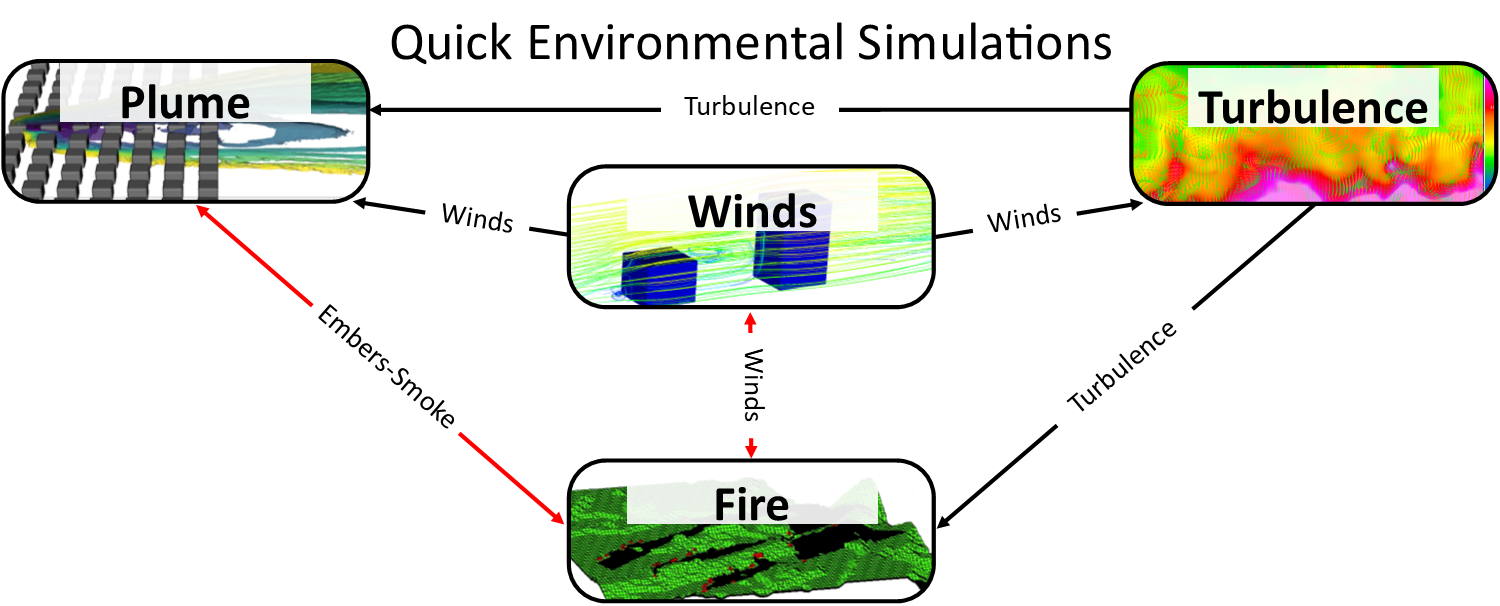
\includegraphics[width=16cm]{Images/QES_chart.png}
\centering
\caption{Schematic of the QUIC EnvSim system and the relationship between different elements of the system including data flow from one element to the other}
\end{figure}

The QES code is a low-computational-cost framework designed to compute high-resolution wind and concentration fields in complex atmospheric-boundary-layer environments. QES is written in C++ and NVIDIA's CUDA for Graphics Processing Unit (GPU) acceleration. The code uses NVIDIA's dynamic parallelism API to substantially accelerate simulations. \textbf{QES requires a NVIDIA GPU with Compute Capability of 7.0 (or higher)}.


\subsubsection{QES-Winds}

QES-Winds is a fast-response 3D diagnostic urban wind model using a mass-conserving wind-field solver \cite{Bozorgmehr2021}. QES-Winds uses a variational analysis technique to ensure the conservation of mass rather than slower yet more physics-based solvers that include the conservation of momentum. QES-Winds minimizes the difference between an initial wind field that is specified using empirical parameterizations and the final wind field. This method requires the solution of a Poisson equation for Lagrange multipliers. The Poisson equation is solved using the Successive Over-Relaxation (SOR) method (an iterative solver), which is a variant of the Gauss-Seidel method with more rapid convergence.

\subsubsection{QES-Turb}

QES-Turb is a turbulence model based on Prandtl’s mixing-length and Boussinesq eddy-viscosity hypotheses. QES-Turb computes the stress tensor using local velocity gradients and some emprical non-local parameterizations.

\subsubsection{QES-Plume}

QES-Plume is a stochastic Lagrangian dispersion model using QES-Winds mean wind field and QES-Turb turbulence fields. QES-Plume solves the generalized Langevin equations to compute the fluctuations of the particle in the turbulent flow fluid. A time-implicit integration scheme is used to solve the Langevin equation, eliminating 'rogue' trajectories. The particles are advanced using a forward Euler scheme. QES-Plume is also a stand-alone dispersion model that can run using fields from diverses sources such as RANS or LES models. 


\subsubsection{QES-Fire}

QES-Fire is a microscale wildfire model coupling the fire front to microscale winds. The model consists of a simplified physics rate of spread model, a kinematic plume-rise model, and a mass-consistent wind solver. The QES-Fire module is currently not publicly available. 
